\documentclass{article}
\usepackage[left=0.5in,top=0.5in,right=0.5in,bottom=0.5in]{geometry}
\usepackage[english]{babel}
\usepackage[utf8]{inputenc}
\usepackage[table]{xcolor}
\usepackage{amssymb,amsmath,amsthm}
\usepackage{changepage,threeparttable}
\usepackage{booktabs,multirow}
\usepackage{graphicx}
\usepackage{soul}
\graphicspath{{./images/}}
\def\F#1{\(#1\)}
\title{Lab 12: The Impedance of an Inductor}
\author{Philip Kim}
\date{\today}
\begin{document}
\maketitle
\vspace*{-1cm}
\begin{table}[!htp]\centering
  \begin{tabular}{|c|c|c|c|c|c|c|}\hline
    \multicolumn{7}{|c|}{\textbf{Table 1: First Approximation for \F{R_{int}}}}\\\hline
    \F{f (Hz)}&s/DIV&\F{V_{RL} (V)}&V/DIV for \F{V_{RL}}&\F{V_{L} (V)}&V/DIV for \F{V_{L}}&\F{R_{int} (\Omega)}\\\hline
    1000& & & & & & \\\hline
  \end{tabular}
\end{table}
\begin{table}[!htp]\centering
  \begin{tabular}{|c|c|c|c|c|c|c|c|c|c|}\hline
    \multicolumn{10}{|c|}{\textbf{Table 2: First Approximation for \F{L}}}\\\hline
    \F{f (Hz)}&s/DIV&\F{V_{RL} (V)}&V/DIV for \F{V_{RL}}&\F{V_{L} (V)}&V/DIV for \F{V_{L}}&\F{I_R (A)}&\F{Z_{L,eff} (\Omega)}&\F{X_L (\Omega)}&L (H)\\\hline
    65000& & & & & & & & & \\\hline
  \end{tabular}
\end{table}
\begin{table}[!htp]\centering
  \begin{tabular}{|c|c|c|c|c|c|}\hline
    \multicolumn{6}{|c|}{\textbf{Table 3: The Impedance of an Inductor}}\\\hline
    \F{f (Hz)}&s/DIV&\F{V_{RL} (V)}&V/DIV for \F{V_{RL}}&\F{V_{L} (V)}&V/DIV for \F{V_{L}}\\\hline
    1000& & & & & \\\hline
    22000& & & & & \\\hline
    32000& & & & & \\\hline
    39000& & & & & \\\hline
    45000& & & & & \\\hline
    50000& & & & & \\\hline
    55000& & & & & \\\hline
    60000& & & & & \\\hline
    65000& & & & & \\\hline
  \end{tabular}
\end{table}
\begin{center}
  \subsection*{Setup}
  % 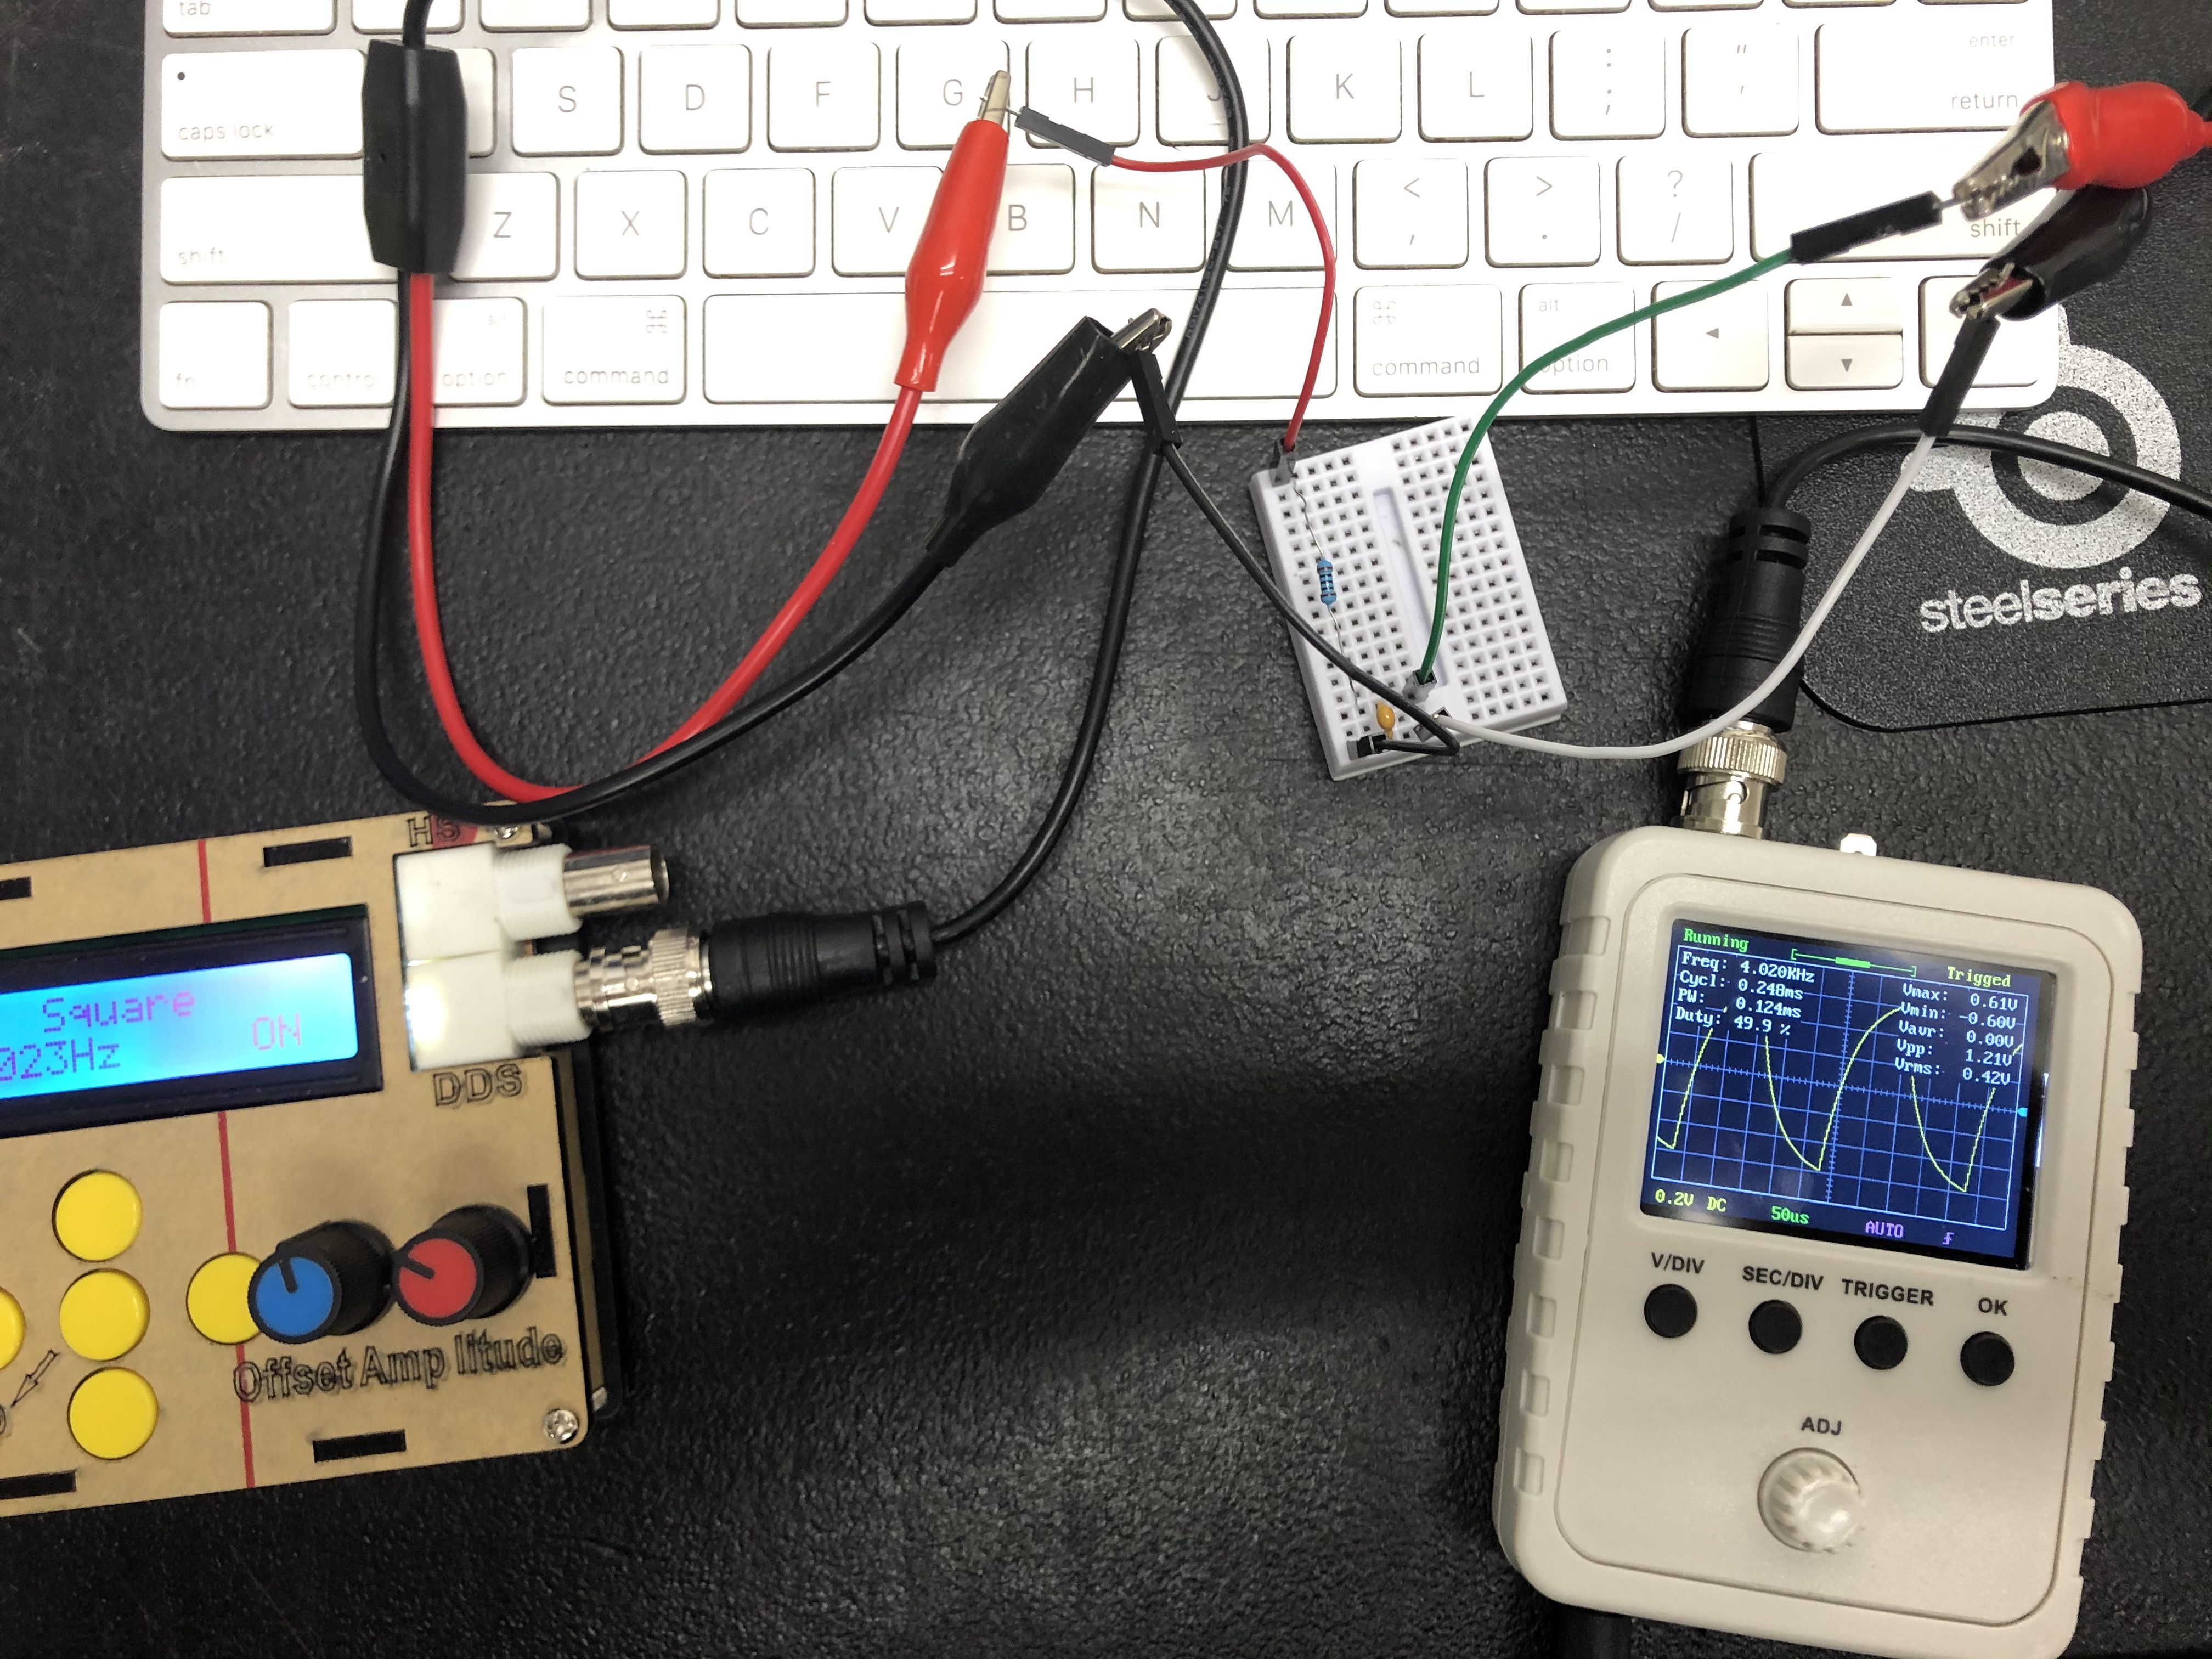
\includegraphics[scale=0.066]{setup1.jpeg}
  setup
  \subsection*{Graph 1}
  % 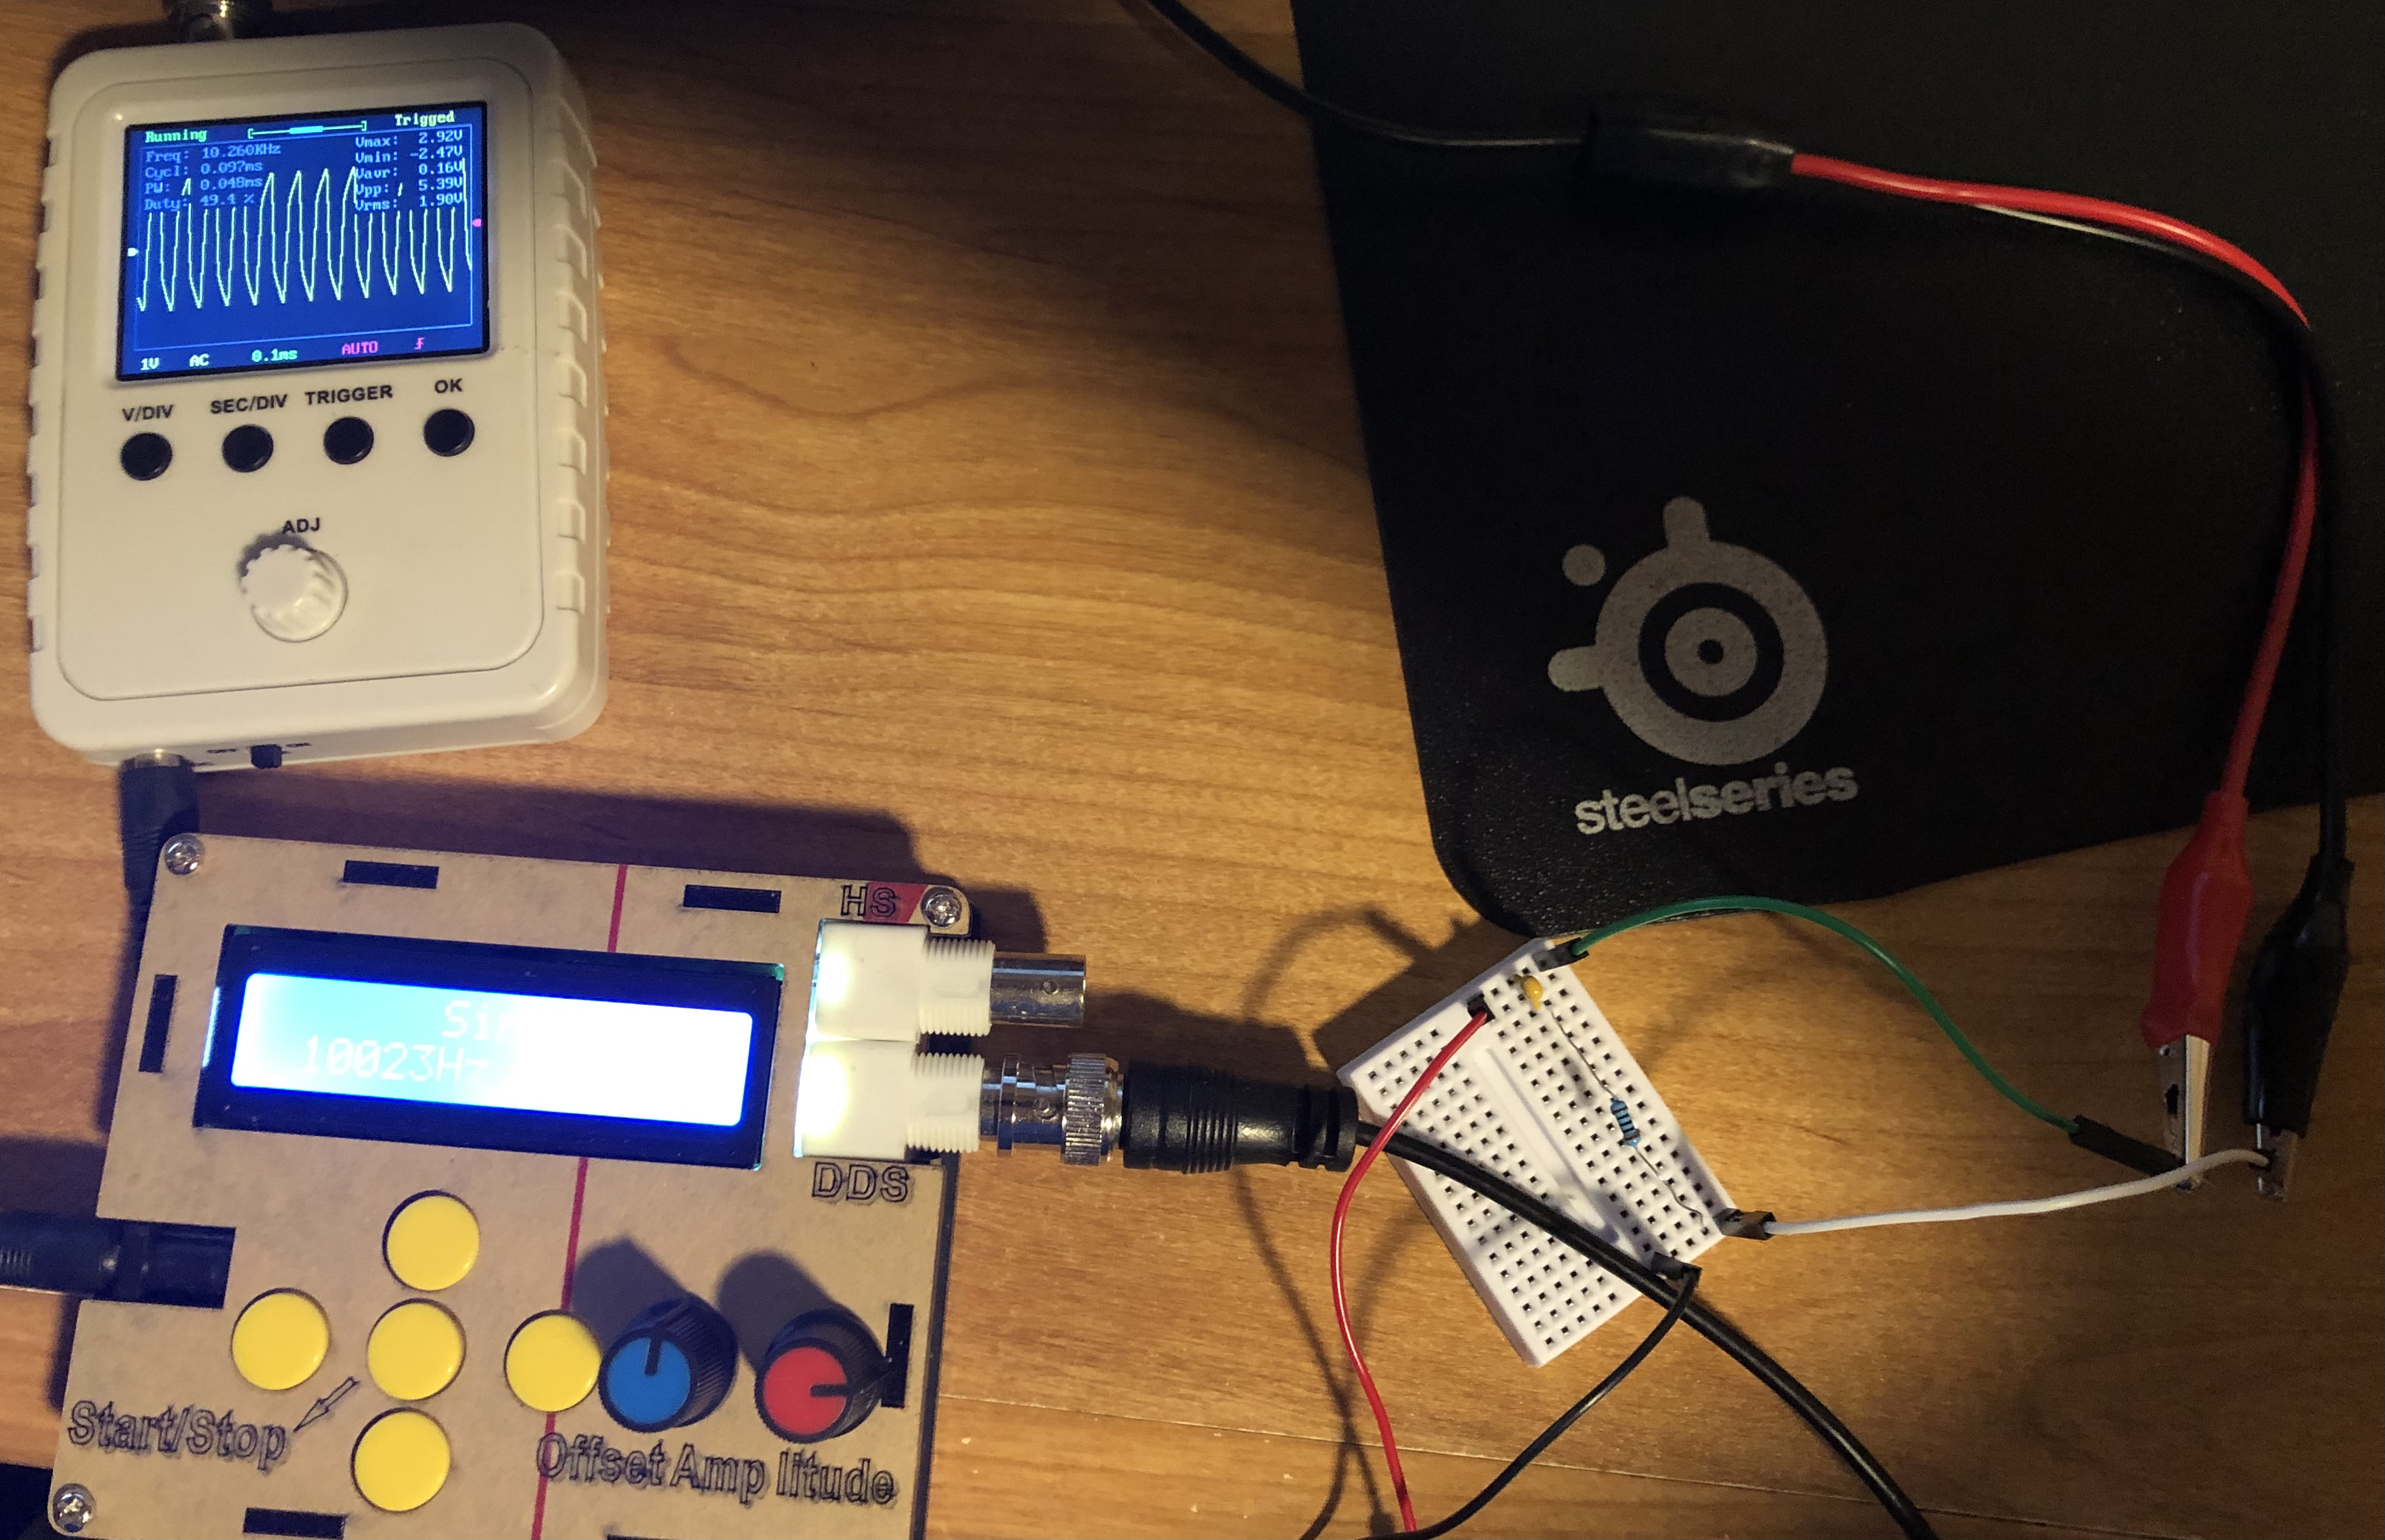
\includegraphics[scale=0.066]{Vrc.jpeg}
  graph 1
  \subsection*{Calculation}
  Calculation
\end{center}
\begin{itemize}
  \item We assume that the current is determined by the largest resistor in the circuit, R. How large is the error that we can expect as a result?
\end{itemize}
\end{document}
